\documentclass[12pt,a4paper,UTF8]{article}
\usepackage{ctex} % Chinese support
\usepackage{graphicx} % Insert images
\usepackage{subfigure}
\usepackage{caption} % to use \caption*
\usepackage{float}
\usepackage{listings} % Print source code
\usepackage{color} % Color support
\usepackage{booktabs} % Professional table support
\usepackage{pdflscape} % Landscape pages support in PDF
\usepackage{hyperref} % Hypertext links support for cross-referencing
\usepackage{amsmath,mathtools}
\usepackage{ulem} % strikethrough

% Customize hyperref format (it's set to no special format here)
\hypersetup{hidelinks}

% Declare directories to search for graphics files for graphicx
\graphicspath{{figures/}}

% Define source code style for listings
\lstdefinestyle{verilog-style}{
	language=Verilog,
	basicstyle=\ttfamily\footnotesize,
	keywordstyle=\bfseries\color[rgb]{0, 0, 1},
	identifierstyle=\color[rgb]{0.5, 0.3, 0.1},
	stringstyle=\color[rgb]{0.6, 0.1, 0.1},
	commentstyle=\itshape\color[rgb]{0.05, 0.5, 0.05},
	backgroundcolor=\color[gray]{0.95},
	numbers=left,
	numbersep=5pt,
	numberstyle=\color[gray]{0.6},
  breaklines=true,
  escapeinside=``
}

\newcommand{\reporttitle}[2]{
  \LARGE\textsf{#1}\quad\underline{\makebox[12em]{#2}}
}

\newcommand{\reportinfo}[2]{
  \large\makebox[4em]{\textsf{#1}}\quad\underline{\makebox[18em]{#2}}
}

\begin{document}
\begin{titlepage}
  \centering
  \vspace*{\fill}
  {\Huge\textsf{数字电路与数字系统实验}} \\ [100pt]
  \reportinfo{实验名称}{exp06 寄存器} \\ [10pt]
  \reportinfo{院系}{计算机科学与技术系} \\ [10pt]
  \reportinfo{学生姓名}{} \\ [10pt]
  \reportinfo{学号}{} \\ [10pt]
  \reportinfo{班级}{数字电路与数字系统实验1班} \\ [10pt]
  \reportinfo{邮箱}{} \\ [10pt]
  \reportinfo{实验时间}{2020 年 9 月 28 日} \\ [10pt]
  \vspace*{\fill}
\end{titlepage}
\tableofcontents
\newpage

\section{实验目的}
\begin{itemize}
  \item 复习寄存器的原理
  \item 学习用Verilog设计寄存器
\end{itemize}

\section{实验原理}
\begin{itemize}
  \item 寄存器的原理:由锁存器和触发器构成的存储电路
  \item 有限域理论和线性反馈移位寄存器反馈方程
\end{itemize}

\section{实验环境/器材}
\begin{itemize}
  \item Quartus编辑器和DE10-Standard开发平台
  \item FPGA开发板
\end{itemize}

\section{程序代码+实验过程+测试方法}
\subsection{实验6.3.1 移位寄存器的实现}
先考虑本实验需要用到的FPGA开发板上的器件。我们需要一个
手动控制的时钟信号,三位的二进制控制位,八位的置数输入,
以及一位串行输入。因此我用FPGA上的按钮来模拟时钟信号和控制位,
用九个开关来模拟置数输入和串行输入。

题目要求很明确,代码直接按要求实现即可:
\begin{lstlisting}[style=verilog-style]
module myLFSR(clk, ctr, load_val, in_data, out_Q);
  input clk, in_data;
  input [2:0] ctr;
  input [7:0] load_val;
  output reg [7:0] out_Q = 8'b0;

  always @ (negedge clk)
    case (ctr)
      // `清0`
      3'd0: out_Q <= 8'b0;
      // `置数`
      3'd1: out_Q <= load_val;
      // `逻辑右移`
      3'd2: out_Q <= {1'b0, out_Q[7:1]};
      // `逻辑左移`
      3'd3: out_Q <= {out_Q[6:0], 1'b0};
      // `算术右移`
      3'd4: out_Q <= {out_Q[7], out_Q[7:1]};
      // LIN
      3'd5: out_Q <= {in_data, out_Q[7:1]};
      // `循环右移`
      3'd6: out_Q <= {out_Q[0], out_Q[7:1]};
      // `循环左移`
      3'd7: out_Q <= {out_Q[6:0], out_Q[7]};
      default: out_Q <= 8'bx;
    endcase
endmodule
\end{lstlisting}

测试文件仅对LIN的情况测试了一下:
\begin{lstlisting}[style=verilog-style]
initial                                                
begin                                                  
	SW[8:0] = 9'b0;
	KEY[3] = 0;
	KEY[2:0] = 3'b101; #2;
	#300;
	$stop;
end

always
begin                                                  
	#0.2 KEY[3] = 1; #5;
	KEY[3] = 0; #4.8;
end

always
begin
	#1 SW[8] = 1; #4;
	SW[8] = 0; #2;
end
\end{lstlisting}

效果如下:
\begin{figure}[H]
  \centering
  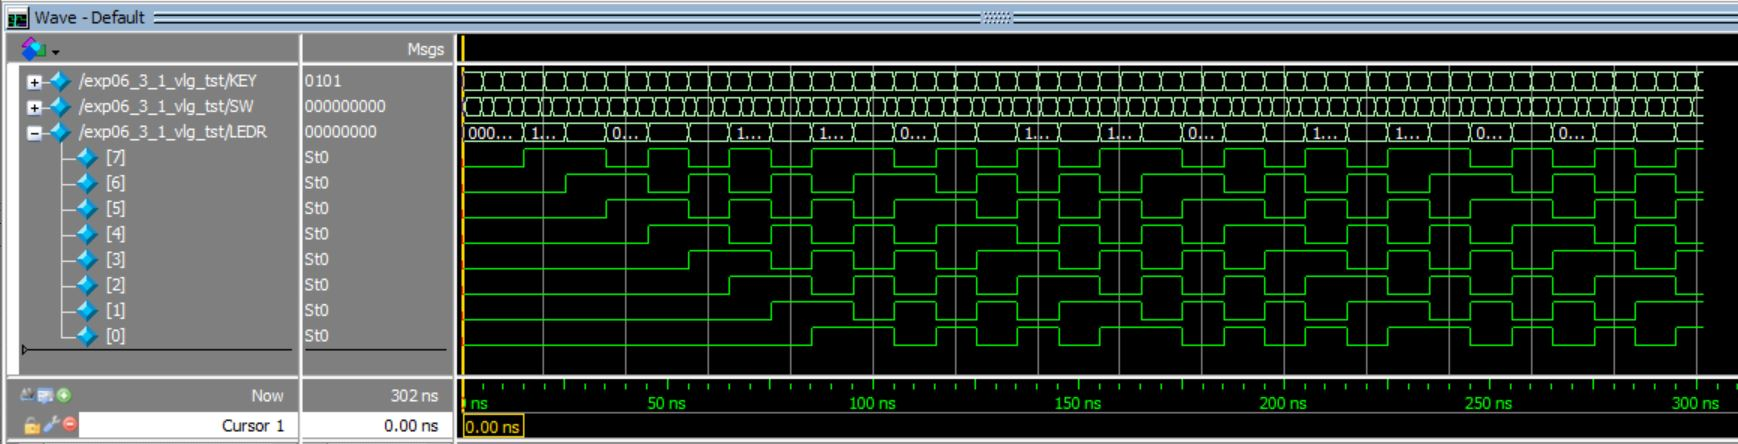
\includegraphics[width=1\textwidth]{1_sim.JPG}
  \caption{仿真运行}
  \label{1_sim}
\end{figure}

\subsection{实验6.3.2 随机数发生器}
这个实验就更简单了。只要用一个按钮模拟时钟,
然后把生成的255种状态的随机数以16进制的形式
显示在数码管上。
\begin{lstlisting}[style=verilog-style]
module random_generator(clk, out_H, out_L);
	input clk;
	output reg [6:0] out_H, out_L;
	reg [7:0] out_binary = 8'b00000001;
	
	always @ (negedge clk)
		out_binary <= {(out_binary[4]^out_binary[3]^out_binary[2]^out_binary[0]),
      out_binary[7:1]};

  always @ (out_binary) begin
    /* `省略七段数码管的case语句` */
  end
endmodule
\end{lstlisting}

反馈方程是根据有限域理论得到的,证明略。

测试代码即让时钟按周期运行,并让程序运行一段时间然后停下来。
这里不贴代码了,直接看仿真结果:
\begin{figure}[H]
  \centering
  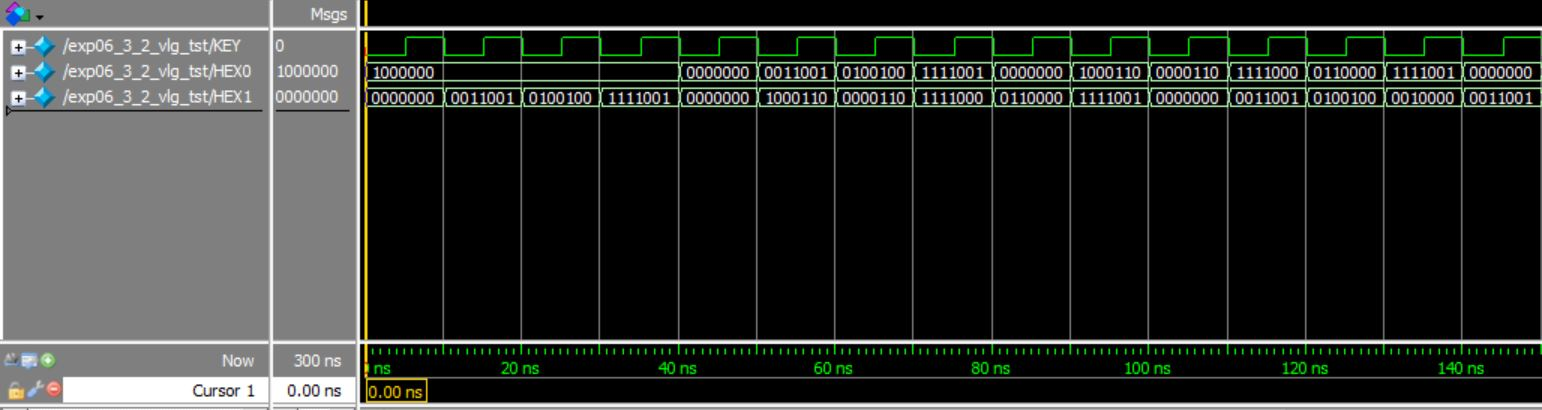
\includegraphics[width=1\textwidth]{2_sim.JPG}
  \caption{仿真运行}
  \label{2_sim}
\end{figure}

\subsection{思考题\quad 更复杂的伪随机数序列}
\subsubsection{比较正确的方法:扩大n}
此方法十分简单粗暴,即把生成随机数序列的位数扩大,然后只取低n位输出。
以本实验为例,我们需要发生n=8位的伪随机数,所以我们可以先设计一个11位
的随机数发生器,然后取低8位输出。

此方法的优点是较难根据生成的伪随机数序列推测出反馈方程。因为反馈方程
产生的值串行输入到最高位,而最高位并不会立即在数码管上显示,需要经过
几个时钟周期的移位才会移到低8位并输出。另外,当我们实际设计的发生器
的位数足够大时,存在反馈方程的参数(操作数)不是低8位的数,例如
$X32=X22\oplus X2\oplus X1\oplus X0$,这会让反馈方程更难推测,
伪随机数序列也就更复杂。

此方法的缺点是空间复杂度与我们实际设计的发生器位数成正相关,所以我们
需要合理安排实际设计的发生器的位数。

\subsubsection{不太正确的方法:缩小n}
{\noindent{\makebox[1em]{\textbullet}}\textsf{初始思路}}

此方法的思路是把n位序列分成多个短序列分别进行随机数发生。

以本实验的n=8为例,我们尝试把它分为两个4位序列分别进行LSFR。
继而我们发现,因为两个序列周期都是$2^4-1=15$个时钟周期,所以
对于其中一个4位序列的任意一种状态$s1$,存在另一个4位序列的
一种状态$s2$,使得$s1$每次出现时,另一个序列的状态必为$s2$。
因此该方法只能生成$2^4-1$种状态而非$2^8-1$种状态。

{\noindent{\makebox[1em]{\textbullet}}\textsf{尝试修改}}

根据这个错误,我们发现,要使两个短序列在发生完$2^8-1$种状态
之前不产生重复,就必须让两个序列各自的状态数互素。

于是我们尝试修改一下这个方法。在此之前我们需要了解一些简单的
\sout{小学数学}知识:
\begin{description}
  \item[梅森素数] 梅森素数指形如$2^p-1$的一类素数。例如
        p=2、3、5、7、13、17、19、31、61、89、107、
        127、521等。目前为止仅发现51个梅森素数。
  \item[循环群] 群是一个具有运算封闭性、运算结合性、
        单位元、逆元的代数系统。若一个群的每一个元素
        都是该群中一个固定元素的幂,则该群为循环群,
        该元素称为该循环群的生成元。n阶循环群生成元的个数
        恰好等于不大于n且与n互质的正整数的个数。
\end{description}
\hspace*{\fill}

记集合$S=\{p_0, p_1, \cdots , p_i, \cdots\}$,该集合中
的元素$p_i$满足$2^{p_i}-1$是梅森素数。我们把n位序列分成
2个长度不同的短序列,其中至少有一个短序列的长度属于$S$,记
该长度为$p_i\in S$的序列为$L1$。另一个序列记为$L2$,其长度
为$x$。记这两个序列的状态数$sp=2^{p_i}-1, sx=2^x-1$。下证
在一个以$sp\times sx$个时钟周期为周期的循环中,这两个序列
拼接成的序列不会有重复值出现。

要证上述引理,我们只要证明在一个$sp\times sx$周期中,
对于$L2$的任意一个状态,该状态每次出现时,$L1$的状态都不同。
即证每过$sx$个时钟周期,取一次$L1$的状态,经过$sp\times sx$
个时钟周期后,取出的$sp$个状态各不相同。这同构于一个模$sp$的
整数加群$G$,根据循环群的相关定理(见上文预备知识),$G$中每个元素
都是生成元。取第$sx(mod\; sp)$个元素作为生成元,构建该群的生成子群$H$。
再根据此时对应的$L2$的状态取$H$的陪集$H'$,由群论的拉格朗日定理
(同构、陪集、拉格朗日定理等知识过于复杂,有兴趣请stfw,这里不解释)
知,$H'=G$,所以这两个序列拼接成的序列不会有重复值出现。

{\noindent{\makebox[1em]{\textbullet}}\textsf{依旧失败}}

但即使这样,所生成的状态数仍然小于$2^n-1$。因为两个序列都没有全零
状态,总共少了$(2^{sp+sx}-1)-(2^{sp}-1)(2^{sx}-1)=2^{sp}+2^{sx}-2$
个状态。为了尽可能往正确方向修改,我们可以修改$L2$的反馈方程使其成为
带有全零状态的发生器。但我们不能修改$L1$,因为修改之后两个序列的状态数
不互素,会导致同初始思路一样的错误。

再次修改之后,我们仍然缺少$L1$为全零状态时的n位序列的状态。
我们只能在$sp\times sx$个时钟周期之外另补缺少的状态,
但这显然会大幅度降低伪随机数的复杂度。为了缝补漏洞,
别无他法,只能做此无奈之举。

\section{实验结果}
实验6.3.1和实验6.3.2都挺好

\begin{figure}[H]
  \centering
  \subfigure{
    \begin{minipage}[H]{0.45\textwidth}
      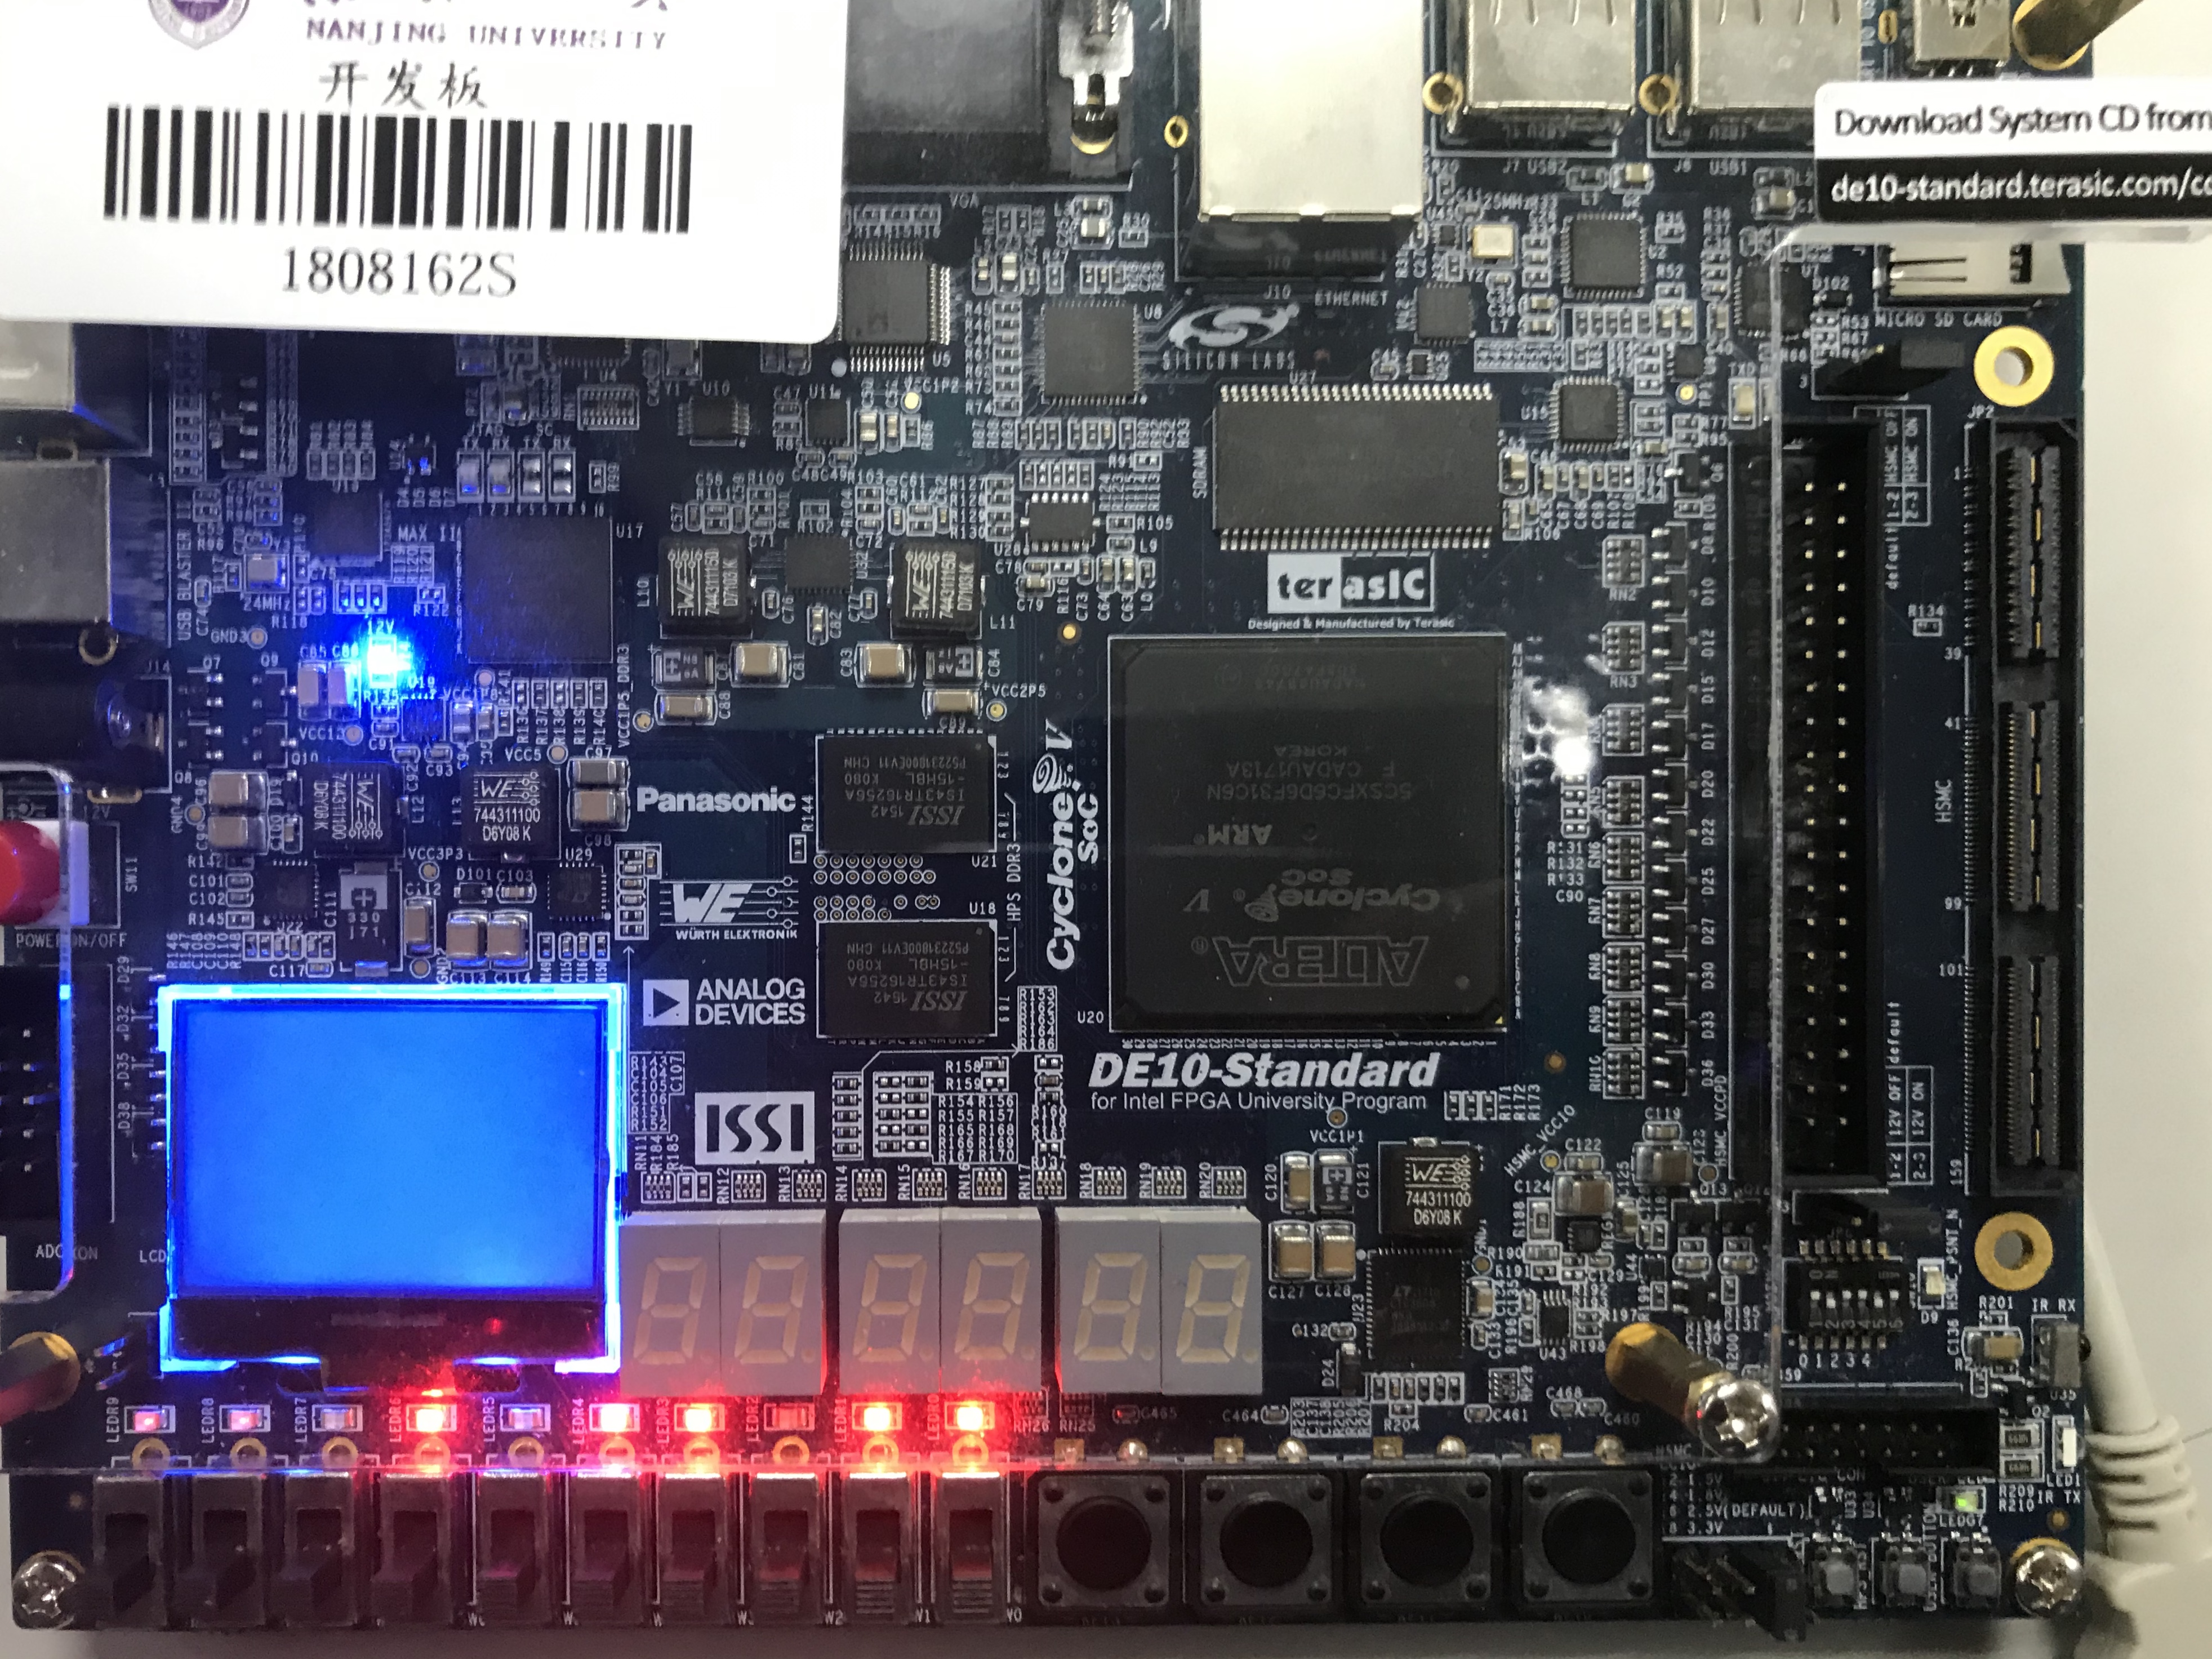
\includegraphics[width=1\textwidth]{1_fpga.JPG}
      \caption*{实验6.3.1}
    \end{minipage}
  }
  \subfigure{
    \begin{minipage}[H]{0.5\textwidth}
      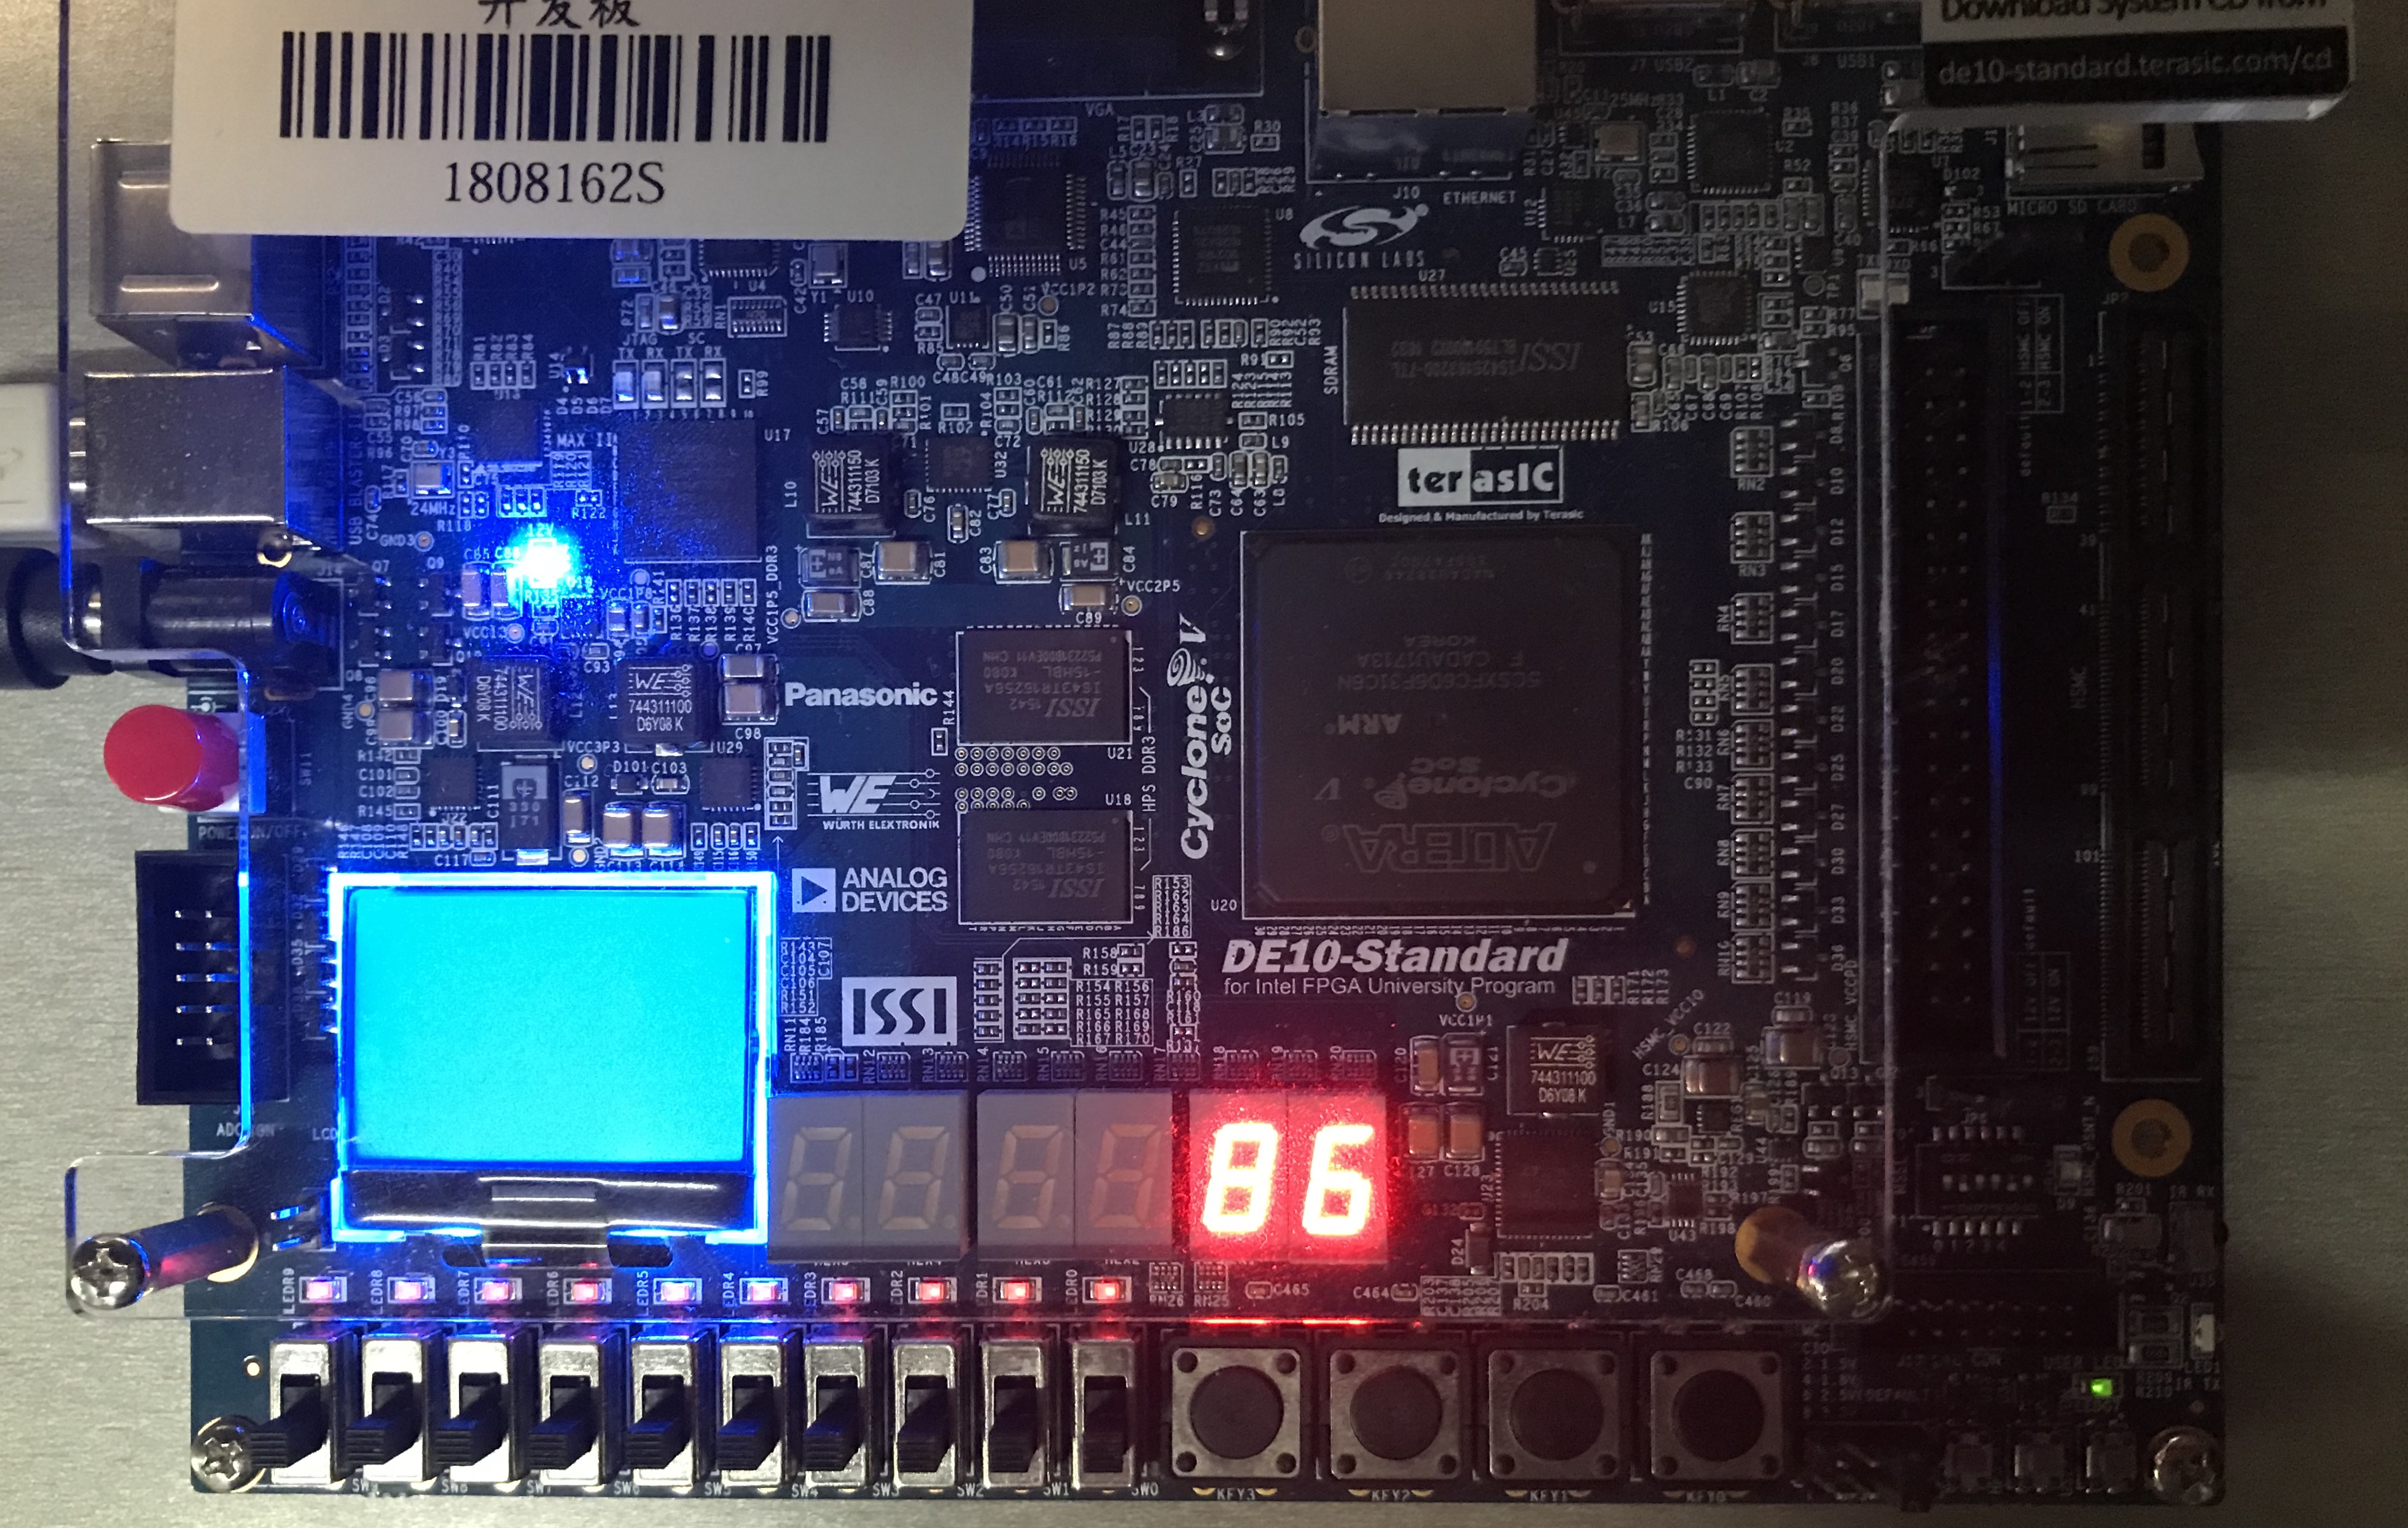
\includegraphics[width=1\textwidth]{2_fpga.JPG}
      \caption*{实验6.3.2}
    \end{minipage}
  }
  \caption{下载运行}
  \label{fpga}
\end{figure}

\section{遇到的问题及解决办法}
\begin{itemize}
  \item 传入子模块的参数的宽度(input [X:Y] var)
        不小心写宽了一位,赋值是按二进制格式赋值的,
        然后在仿真运行的时候就一直仿真不出来(输出值
        是一条红线,值不确定)。这种情况不会出现报错,
        只会出现在警告里。得到的教训是如果有de不出来
        的bug,不能因为没报错就不去看控制台输出,
        一定要去看提示的警告信息
\end{itemize}

\section{得到的启示}
\begin{itemize}
  \item 写bug的时候warnings一定要看啊一定要看(重要的事情说n遍)
  \item 数学证明让人心力交瘁
\end{itemize}

\section{意见和建议}
\begin{itemize}
  \item ``按键消抖''说明文档中倒数第二段应该是``实验4 锁存器和触发器''
\end{itemize}

\end{document}